\chapter{Results, Evaluation and Discussion}
\label{chapter4}

This chapter reports the experimental evaluation of the simulation framework described in Chapters~\ref{chapter2} and~\ref{chapter3}. Section~\ref{sec:results-setup} documents the experimental setup and the matrix of configurations. Section~\ref{sec:results-main} presents the results on segment based reservation. Section~\ref{sec:results-runtime} analyses the computational cost of the policies. Section~\ref{sec:results-variation} summarises supplementary experiments. Section~\ref{sec:results-findings} discusses the broader algorithmic findings. Section~\ref{sec:results-limitations} outlines the limitations of the evaluation. Section~\ref{sec:results-conclusions} draws conclusions from the experimental data. Finally, Section~\ref{sec:results-future} identifies directions for future work.

\section{Experimental setup}
\label{sec:results-setup}

The main experiment that took place was a sweep over the eight policies and the binary \texttt{allow\_predicted\_}\allowbreak\texttt{collisions} toggle introduced in Chapter~\ref{chapter2}, at two simulation durations and across five seeds. Each configuration was executed twice to verify determinism. Three supplementary experiments hold the policy set fixed and vary one independent variable at a time. These were fleet size, obstacle density and the rate of delivery jobs. Table~\ref{tab:experiment-matrix} summarises the experiment matrix.

\begin{table}[h]
\centering
\caption{Experimental matrix.}
\label{tab:experiment-matrix}
\begin{tabular}{|p{0.15\textwidth}|p{0.08\textwidth}|p{0.18\textwidth}|p{0.05\textwidth}|p{0.10\textwidth}|p{0.24\textwidth}|}\hline
Main sweep & 100, 500 & 42, 53, 82, 97, 23 & 2 & All 8 & \texttt{allow\_predicted\_} \newline \texttt{collisions} \\
\hline
Long run & 1000 & 42, 53, 82 & 2 & Greedy, A* & \texttt{allow\_predicted\_} \newline \texttt{collisions} \\
\hline
Fleet scale & 100 & 42 & 1 & All 8 & Number of UAVs \\
\hline
Obstacle density & 100 & 42 & 1 & All 8 & Obstacle proportion \\
\hline
Spawn rate & 100 & 42 & 1 & All 8 & Poisson rate $\lambda$ \\
\hline
\end{tabular}
\end{table}

Five metrics are recorded per configuration. Completion rate is the proportion of jobs delivered within the simulation time limit. Average delivery time is the mean simulated elapsed time between job assignment and delivery (in seconds). Total collisions (recorded by the ASP through the continuous collision check). Minimum separation is the smallest distance between two UAVs observed during the simulation, in metres. Runtime is the real world time it took to run the simulation, it will be used as a proxy for computational cost. 

Five seeds is the minimum required for a meaningful descriptive comparison. The Results are reported as means across these seeds. The supplementary experiments use a single seed and therefore only observations. The frameworks deterministic execution, verified empirically in Chapter~\ref{chapter3} by re running every configuration with bit identical results, supports the reproducibility of every figure presented in this chapter.

\section{Effect of the reservation mechanism}
\label{sec:results-main}

Figure~\ref{fig:main-comparison} presents the comparison of the eight policies under both states of the \texttt{allow\_predicted\_}\allowbreak\texttt{collisions} toggle at sim\_time = 500\,s, averaged across the five seeds.

\begin{figure}[h]
\centering
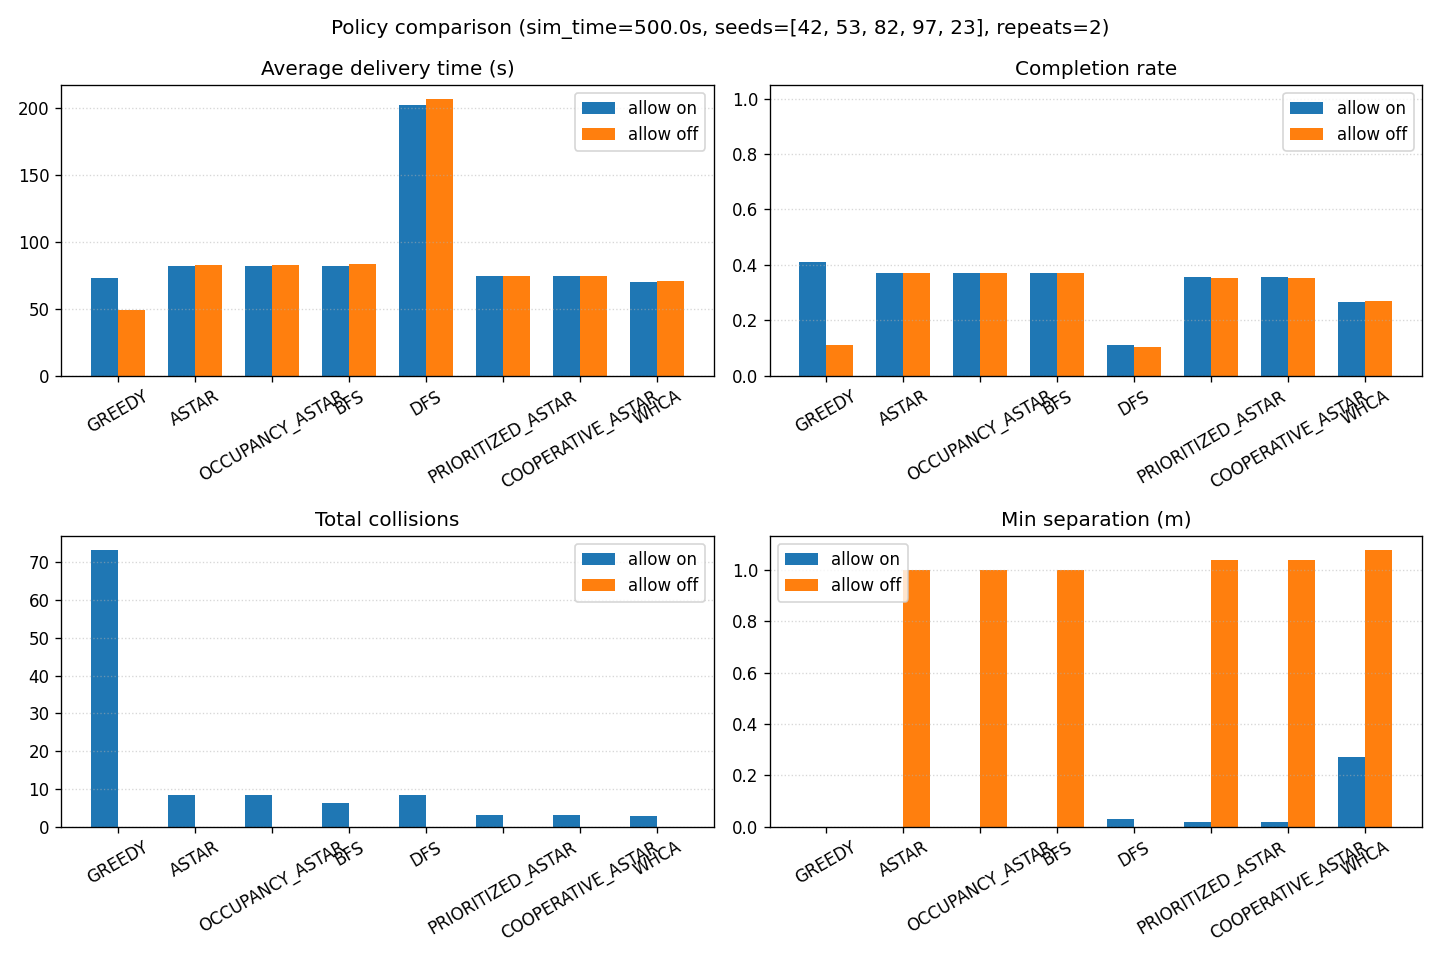
\includegraphics[width=\textwidth]{figures/policy_comparison_t500.png}
\caption{Policy comparison at sim\_time = 500\,s, seeds \{42, 53, 82, 97, 23\}, two repeats per configuration. Blue bars: \texttt{allow\_predicted\_}\allowbreak\texttt{collisions = True} (``allow on''); orange bars: \texttt{allow\_predicted\_}\allowbreak\texttt{collisions = False} (``allow off'').}
\label{fig:main-comparison}
\end{figure}

The total collisions graph shows the central finding that this project aims to demonstrate. With the reservation mechanism advisory (allow on), Greedy averages 73 collisions per run, A*, Occupancy A*, BFS, and DFS average between six and nine, and Prioritised A*, Cooperative A*, and WHCA* average three. But, when the mechanism is toggled, every policy averages zero collisions (and the pre averaged data shows 0). The reservation mechanism therefore constructively prevents UAV on UAV collisions. 

The completion rate graph shows that the reservation mechanism causes a large fall in Greedy's completion rate, but almost no change for other policies (All other policies are essentially unchanged: A*, Occupancy A*, and BFS hold at approximately 0.37; Prioritised A* and Cooperative A* at approximately 0.35; WHCA* at approximately 0.27; and DFS at approximately 0.10). This is entirely down to the fact that no other policy will submit a reservation that intersects a static obstacle which means that the ASP will reject the reservation and UAVs using the greedy policy will fail cuaseing the UAV to escalate through \texttt{HOVER\_WAIT} to \texttt{EMERGENCY}.  

The average delivery time panel shows the same issue. Greedy's allow on delivery time of 73\,s drops to 50\,s under allow off, reflecting that the few deliveries Greedy completes under enforcement are short, low-conflict routes. longer routes are rejected and never recorded. All other policies show essentially no difference in delivery time between the two states.

\section{Computational cost}
\label{sec:results-runtime}

Figure~\ref{fig:runtime-comparison} presents the real world runtime of each policy at sim\_time = 500\,s under both toggle states.

\begin{figure}[h]
\centering
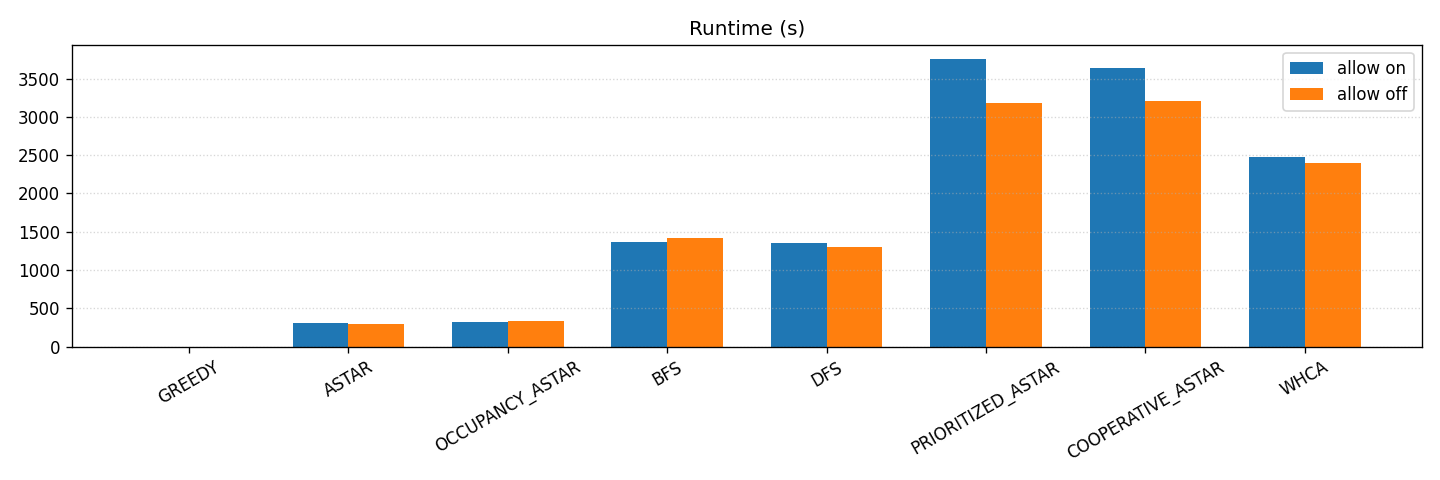
\includegraphics[width=\textwidth]{figures/policy_runtime_comparison_t500.png}
\caption{Wall-clock simulation runtime in seconds at sim\_time = 500\,s, seeds \{42, 53, 82, 97, 23\}, two repeats per configuration.}
\label{fig:runtime-comparison}
\end{figure}

The runtimes span three orders of magnitude. Greedy runs in essentially zero time because it performs no search. Then its informed search A* and Occupancy A* that run in approximately 300\,s. After this its BFS and DFS run in approximately 1{,}300--1{,}400\,s, reflecting their uninformed exploration. Then finally reservation based policies are the most expensive, Prioritised A* and Cooperative A* run in approximately 3{,}200--3{,}800\,s, and WHCA* in approximately 2{,}400\,s. This therefor shows that the cost of reservation based coordination is approximately 10x to A* and approximately 20x  to Greedy. WHCA* is an outlier in the patter and it shows a lower runtime than the other reservation polices, which is likely due to its bounded horizen.

\section{Behaviour under varying conditions}
\label{sec:results-variation}

The three single seeded supplementary experiments examine fleet size, obstacle density, and demand intensity at sim\_time = 100\,s. They are reported as descriptive observations rather than statistically rigorous findings (due to the single seed and the short simulation time).

Despite varying fleet size between small, medium, and large it produces essentially identical completion rates of approximately 0.14 for every policy (except DFS due to its massively inefficient nature). Completion rate at is therefore not limited by fleet capacity therefore adding more UAVs does not produce more deliveries. The bottleneck is elsewhere in the system, i belive it to be both depot take off and landing and also gate capcaity. Despite no decrese in delivery time with fleet size, the run time however does increase with fleet size for all polices (such as WHCA* going from 45\,s to 78\,s). This is an expected result as more UAVs means that more searches/ routes are needed to be generated. Other than WHCA* and BFS other polices show increases that are approximately linear to the number of UAVs.

In an obstacle-heavy world, the same pattern produced (albeit at a smaller scale)  Completion rate is reduced to approximately 0.06 across policies (from 0.14--0.40 in th default), reflecting that higher obstacle density makes more routes infeasible.
